\documentclass[12pt]{article}
\usepackage{graphicx}

\begin{document}
\title{Lab5 - Bayesian Networks}
\author{Maxime Lhoustau and Philipp Schlieker}
\maketitle

\section*{General Information}
$A$ = "Person has recently visited Asia"\\
$S$ = "Person is a smoker"\\
$T$ = "Person has tuberculosis"\\
$L$ = "Person complains about lung problems"\\
$C$ = "Person has cancer"\\
$B$ = "Person has only a bronchitis"\\
$ST$ = "Stethoscope test is positive"\\
$X$ = "X-Ray is positive"\\
$P(A) = 10 \%$\\
$P(S) = 30 \%$\\
$P(T|A) = 10 \%$\\
$P(T|\bar{A}) = 1 \%$\\
$P(C|S) = 20\%$\\
$P(C|\bar{S}) = 2\%$\\
$P(\bar{C},\bar{T},B|\bar{S}) = 80\%$\\
$P(\bar{C},\bar{T},B|S) = 60\%$\\
\\
\begin{tabular}{|c|c|cc|}
\hline
 & & \multicolumn{2}{|c|}{ST} \\
B&C&F&T\\
\hline
T&T&&60\%\\
T&F&&60\%\\
F&T&&60\%\\
F&F&99\%&\\
\hline
\end{tabular}

\begin{tabular}{|c|c|cc|}
\hline
 & & \multicolumn{2}{|c|}{X} \\
T&C&F&T\\
\hline
T&T&&70\%\\
T&F&&70\%\\
F&T&&70\%\\
F&F&98\%&\\
\hline
\end{tabular}
\newpage
\section{Model this problem using a Bayesian network}
\begin{figure}[hbtp]
\caption{Bayesian Network}
\centering
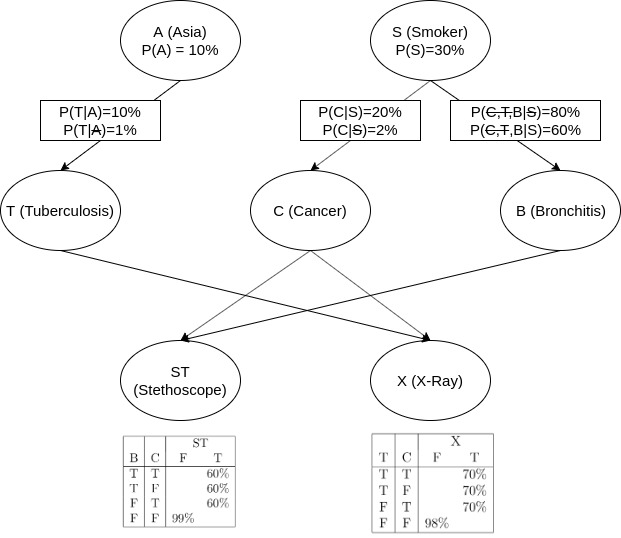
\includegraphics[scale=.7]{network.jpg}
\end{figure}
\section{If the patient is not smoking and has not recently visited Asia, can you infer with disease?}
No, it is not possible to infer the disease with 100\% certainty. The disease with the highest probability is Bronchitis.\\
$P(\bar{A}, \bar{S}, T) = P(T|\bar{A},\bar{S}) * P(\bar{A}|\bar{S}) * P(\bar{S}) = 0.01 * 0.9 * 0.7 = 6.3\%$\\
$P(\bar{A}, \bar{S}, C) = P(C|\bar{A},\bar{S}) * P(\bar{A}|\bar{S}) * P(\bar{S}) = 0.02* 0.9 * 0.7 = 12.6\%$\\
$P(\bar{A}, \bar{S}, B) \geq P(\bar{A}, \bar{S}, B, \bar{T}, \bar{C}) = P(B,\bar{T}, \bar{C} |\bar{A},\bar{S}) * P(\bar{A}|\bar{S}) * P(\bar{S}) = 0.8 * 0.9 * 0.7 = 50.4\%$\\
\section{According to the disease inferred in Point 2, the doctor decides to auscultate the patient's lungs with a stethoscope? Why?}
In order to decide whether the person has a Bronchitis this test is helpful. If the person has a bronchitis, than it is highly likely that he will not have cancer and tuberculosis.\\
\section*{The stethoscope test is negative. What is the new inferred diagnosis?}
The disease with the highest likelihood is now tuberculosis.\\
$ P(\bar{A}, \bar{S}, C, \bar{ST}) = P(\bar{A}, \bar{S}, C) * P(C | \bar{ST}) = 12.6\% * 1\% = 0.126\% $\\
$ P(\bar{A}, \bar{S}, B, \bar{ST}) = P(\bar{A}, \bar{S}, B) * P(C | \bar{ST}) = 50.4\% * 1\% = 0.504\% $\\
$P(\bar{A}, \bar{S}, T, \bar{ST}) = P(\bar{A}, \bar{S}, T) = 6.3\%$
\section{The doctor orders an X-Ray. The X-Ray test is positive. What is the new inferred diagnosis?}
Tuberculosis\\
\begin{figure}[hbtp]
\centering
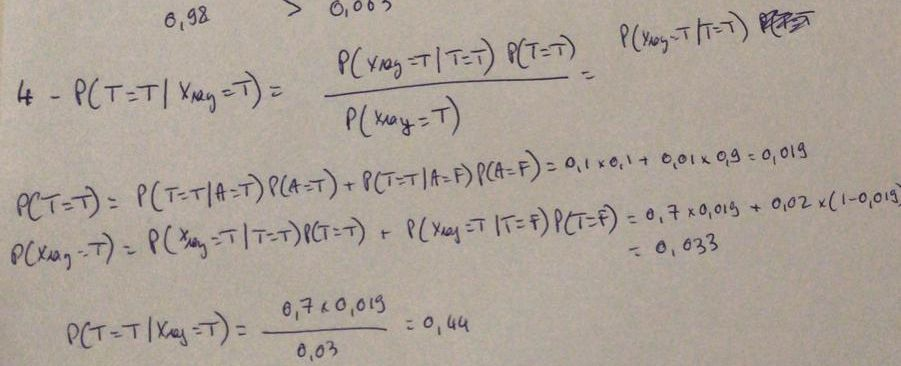
\includegraphics[scale=.45]{lab5_ex4.jpeg}
\end{figure}
\section{Was the X-Ray needed?}
The X-Ray increased the certainty.
\end{document}
